\documentclass[10pt,a4paper]{article}
\usepackage[utf8]{inputenc}
\usepackage{graphicx}
\author{renatolrr}
\title{Polarización universal o por divisor de tensión}
\begin{document}
\maketitle
Vamos a calcular el siguiente circuito:

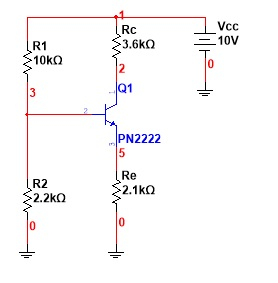
\includegraphics[scale=1]{Images/Imagen1.jpg} 

Para el análisis sustituimos el divisor resistivo por el equivalente de Thevénin entre la base y la masa.

\section{Equivalente Thévenin}
\subsection{Calculo de $R_{0}$}
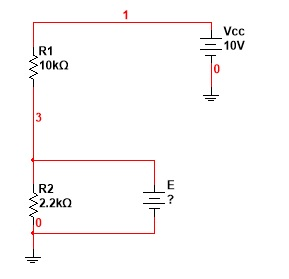
\includegraphics[scale=1]{Images/Imagen2.jpg}
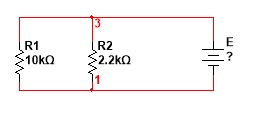
\includegraphics[scale=1]{Images/Imagen3.jpg} 
\\
Con Vcc en corto tenemos que calcular Ro
\[R=E/I\]
Si nos fijamos son las dos resistencias en paralelo, luego la resistencia equivalente es:
\[R_{0}=\frac{R_{1}*R_{2}}{R_{1}*R_{2}}\]
Por lo tanto tenemos en nuestro caso:
\[R_{0}=R_bb=\frac{10K*2.2k}{10K*2.2K}\]
\subsection{Calculo de $E_{0}$}
La intensidad de base es cero por lo tanto tenemos:
\begin{center}
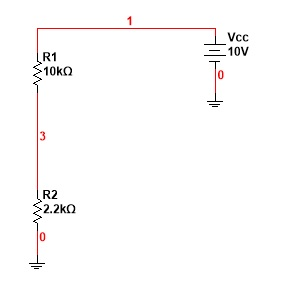
\includegraphics[scale=1]{Images/Imagen4.jpg}
\end{center}
Y calculamos $E_{0}$
\[E_{o}=\frac{V_{cc}}{R_{1}+R_{2}}*R_{2}\]
En nuestro caso 
\[E_{o}=V_{bb}=\frac{10V}{10K+2.2K}*2.2K=1.8V\]
\subsection{Circuito equivalente}
A partir de este momento utilizamos el circuito equivalente:
\\
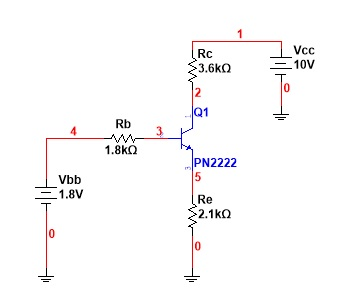
\includegraphics[scale=1]{Images/Imagen5.jpg}
\section{Valores de la intensidad y del voltaje}
\subsection{Ecuaciones fundamentales}
\begin{equation}
I_{e}=I_{c}+I_{b}
\end{equation}
\begin{equation}
I_{c}=\beta*I_{b}
\end{equation}
\subsection{Malla base}
Si consideramos la malla base tenemos:
\begin{center}
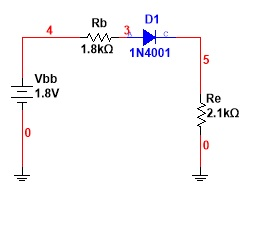
\includegraphics[scale=1]{Images/Imagen6.jpg}
\end{center}
Luego se tiene:
\begin{equation}
V_{bb}=I_{b}R_{b}+V_{be}+I_{e}R_{e}
\end{equation}

\end{document}